%%%%%%%%%%%%%%%%%%%%%%%%%%%%%%%%%%%%%%%%%%%%%%%%%%%%%%%
\documentclass{article}
%%%%%%%%%%%%%%%%%%%%%%%%%%%%%%%%%%%%%%%%%%%%%%%%%%%%%%%
\usepackage[utf8]{vietnam}
%%%%%%%%%%%%%%%%%%%%%%%%%%%%%%%%%%%%%%%%%%%%%%%%%%%%%%%
\usepackage{graphicx}
%%%%%%%%%%%%%%%%%%%%%%%%%%%%%%%%%%%%%%%%%%%%%%%%%%%%%%%
\usepackage{hyperref}
%%%%%%%%%%%%%%%%%%%%%%%%%%%%%%%%%%%%%%%%%%%%%%%%%%%%%%%
\usepackage{xcolor}
\pagecolor[RGB]{40, 42, 54} % Đặt màu nền
\color[RGB]{18, 161, 24} % Đặt màu chữ
%%%%%%%%%%%%%%%%%%%%%%%%%%%%%%%%%%%%%%%%%%%%%%%%%%%%%%%
\usepackage{float} % Cố định hình ảnh [H]
%%%%%%%%%%%%%%%%%%%%%%%%%%%%%%%%%%%%%%%%%%%%%%%%%%%%%%%
\begin{document}
%%%%%%%%%%%%%%%%%%%%%%%%%%%%%%%%%%%%%%%%%%%%%%%%%%%%%%%
\tableofcontents
\newpage
%%%%%%%%%%%%%%%%%%%%%%%%%%%%%%%%%%%%%%%%%%%%%%%%%%%%%%%
\listoffigures
\newpage
%%%%%%%%%%%%%%%%%%%%%%%%%%%%%%%%%%%%%%%%%%%%%%%%%%%%%%%
\section{Tuần 3: Xây dựng dashboard}
%%%%%%%%%%%%%%%%%%%%%%%%%%%%%%%%%%%%%%%%%%%%%%%%%%%%%%%
\subsection{Bài 1}

\subsubsection{Thực hành tạo dashboard theo video}

\begin{figure}[H]
\centering
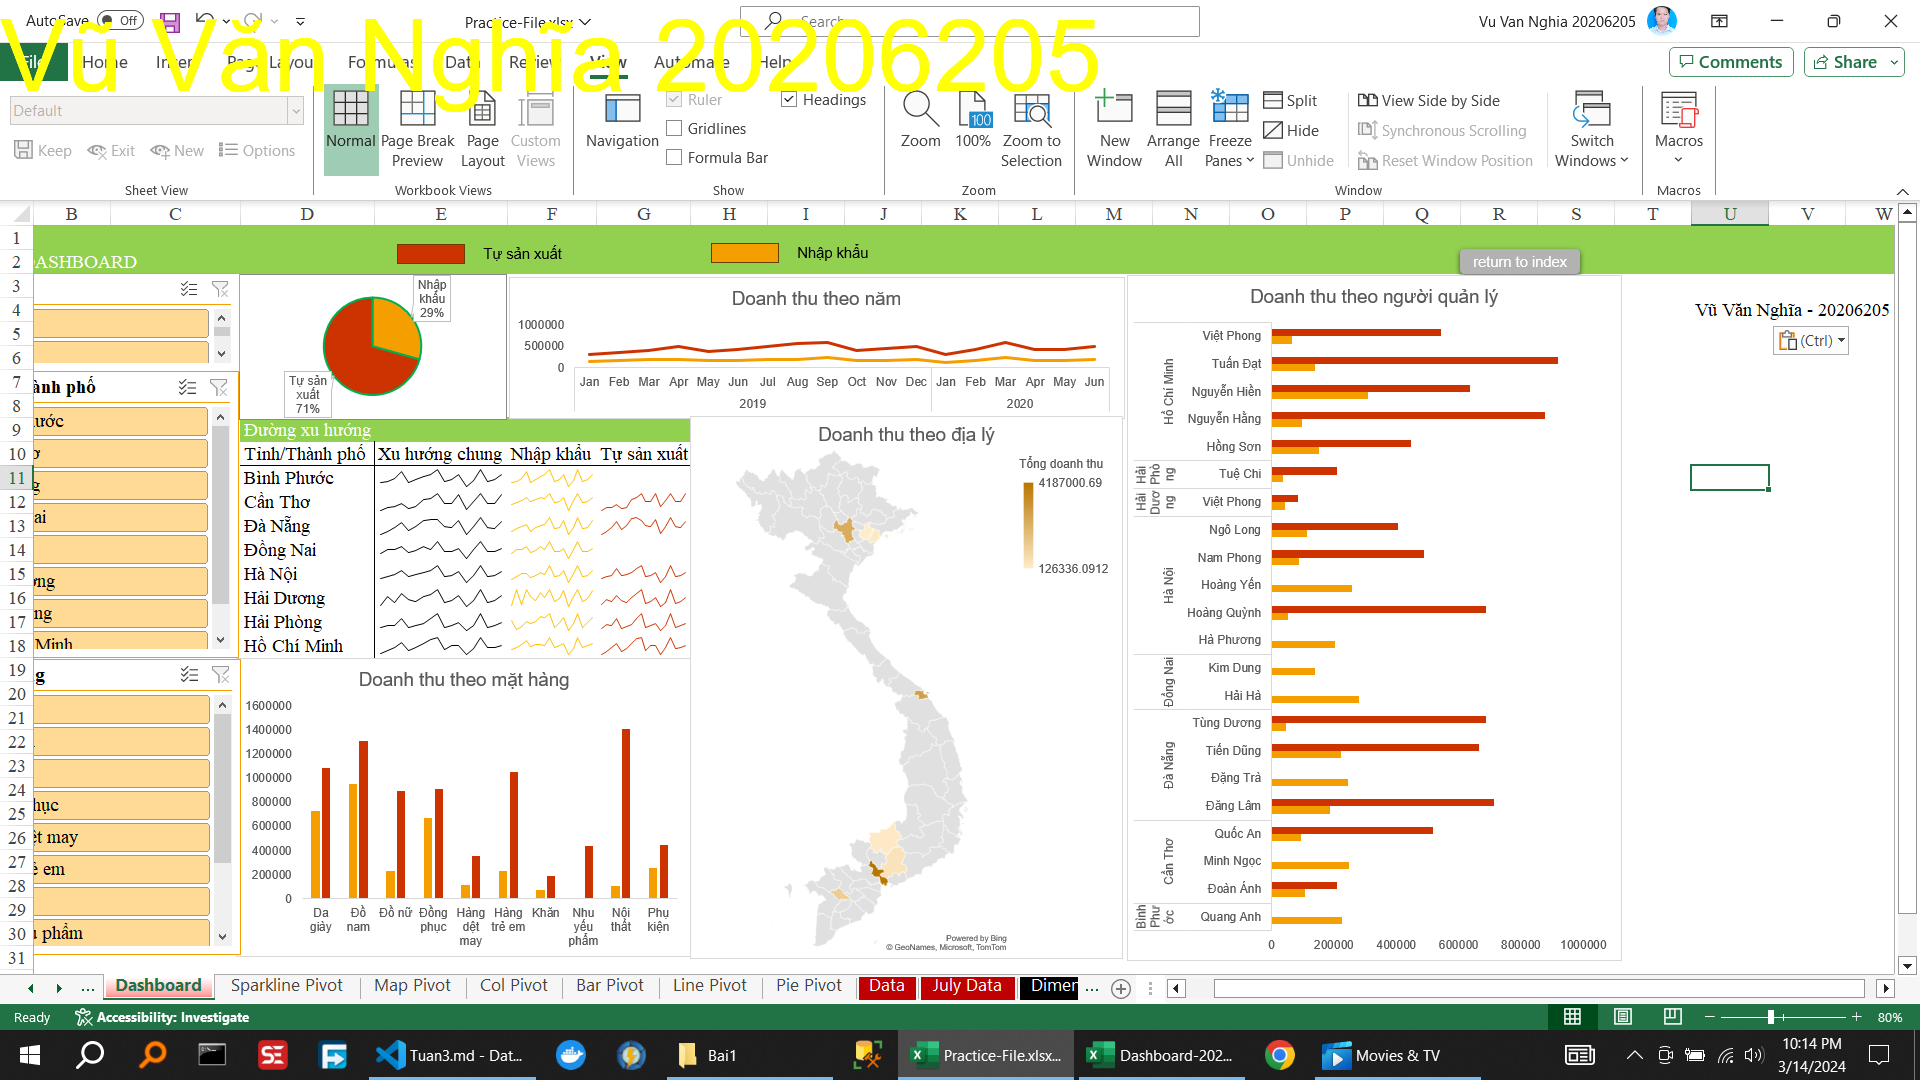
\includegraphics[scale = 0.15]{Bai1/ThucHanh/0.png}
\caption{Thực hành tạo dashboard theo video}
\end{figure}

\subsubsection{Thực hành phân tích dashboard}

\begin{itemize}
\item Đọc dashboard và phân tích
\begin{itemize}
\item Dashboard dùng để mô tả về doanh số bán hàng cho thị trường Việt Nam.
\item Dashboard có các biểu đồ:
\begin{itemize}
\item Biểu đồ tròn: thể hiện tỷ lệ nhập khẩu và tự sản xuất.
\item Biểu đồ đường: thể hiện doanh thu theo năm.
\item Biểu đồ thanh: thể hiện doanh thu theo người quản lý.
\item Biểu đồ cột: thể hiện doanh thu theo mặt hàng.
\item Biểu đồ bản đồ: thể hiện doanh thu theo địa lý.
\end{itemize}
\end{itemize}
\item Xác định các chiều (DIM), các các yếu tố phân tích (FACT)

\begin{figure}[H]
\centering

\includegraphics[scale = 0.15]{Bai1/ThucHanh/DIM-FACT.excalidraw.png}
\caption{Thực hành xác định các chiều (DIM), các các yếu tố phân tích (FACT)}
\end{figure}

\begin{itemize}
\item DIM: Thời gian, Năm, Loại hình Sản xuất, Tỉnh/Thành phố, Nước, Quản lý, Mặt hàng, Khách hàng.
\item FACT: Doanh số (Triệu).
\end{itemize}

\item Sử dụng công cụ Remove Duplicate để tạo ra con voi khái niệm các chiều.

\begin{figure}[H]
\centering
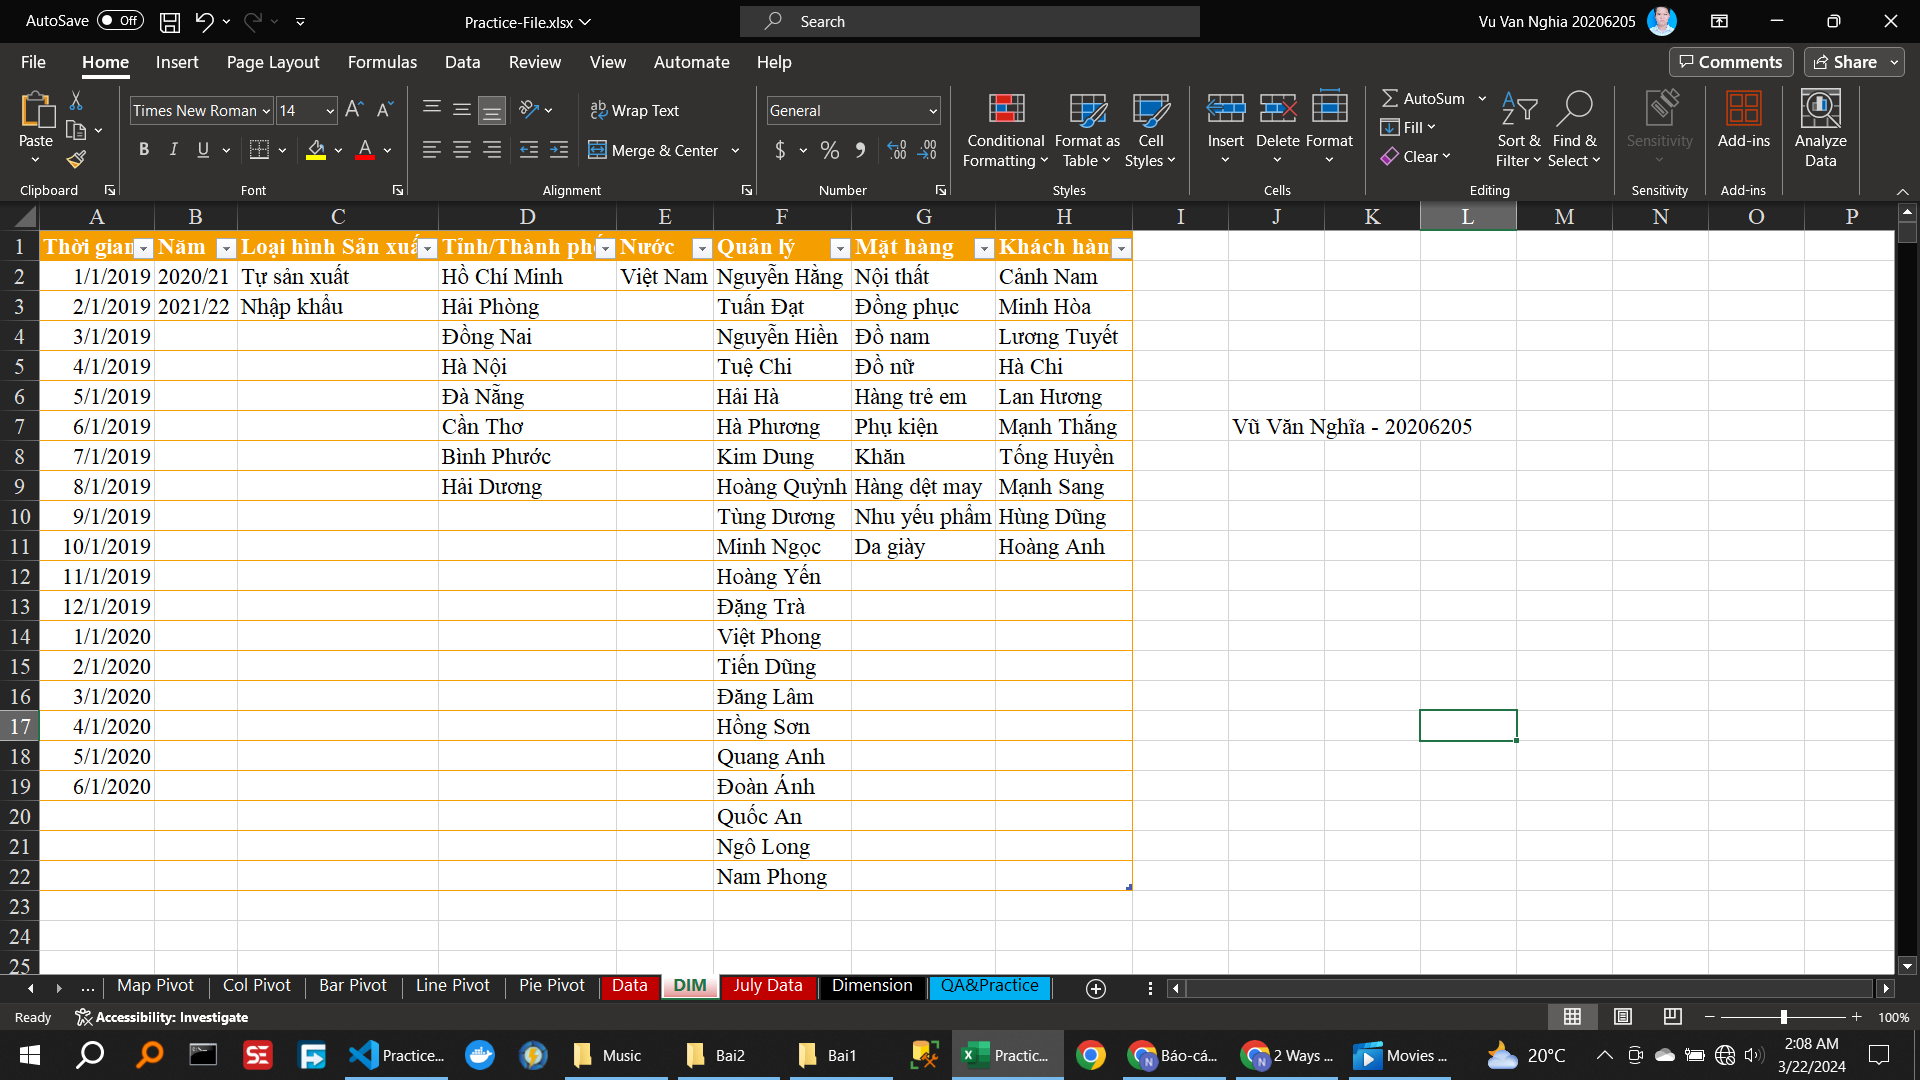
\includegraphics[scale = 0.15]{Bai1/ThucHanh/VOI.png}
\caption{Thực hành sử dụng công cụ Remove Duplicate để tạo ra con voi khái niệm các chiều}
\end{figure}

\end{itemize}

%%%%%%%%%%%%%%%%%%%%%%%%%%%%%%%%%%%%%%%%%%%%%%%%%%%%%%%
\subsection{Bài 2}

 \subsubsection{ Viết Requirement cần phân tích}
 Các yêu cầu phân tích:

 \begin{itemize}
\item      Tổng doanh thu theo giảm giá
\item      Tình trạng đơn hàng
\item      Doanh thu theo địa lý
\item      Tổng số lượng đơn hàng
\item      Tổng số lượng khách hàng
\item      Tổng số lượng đơn hàng
    \end{itemize}

    \subsubsection{ Xác định các DIM, FACT}


    \begin{figure}[H]
        \centering
        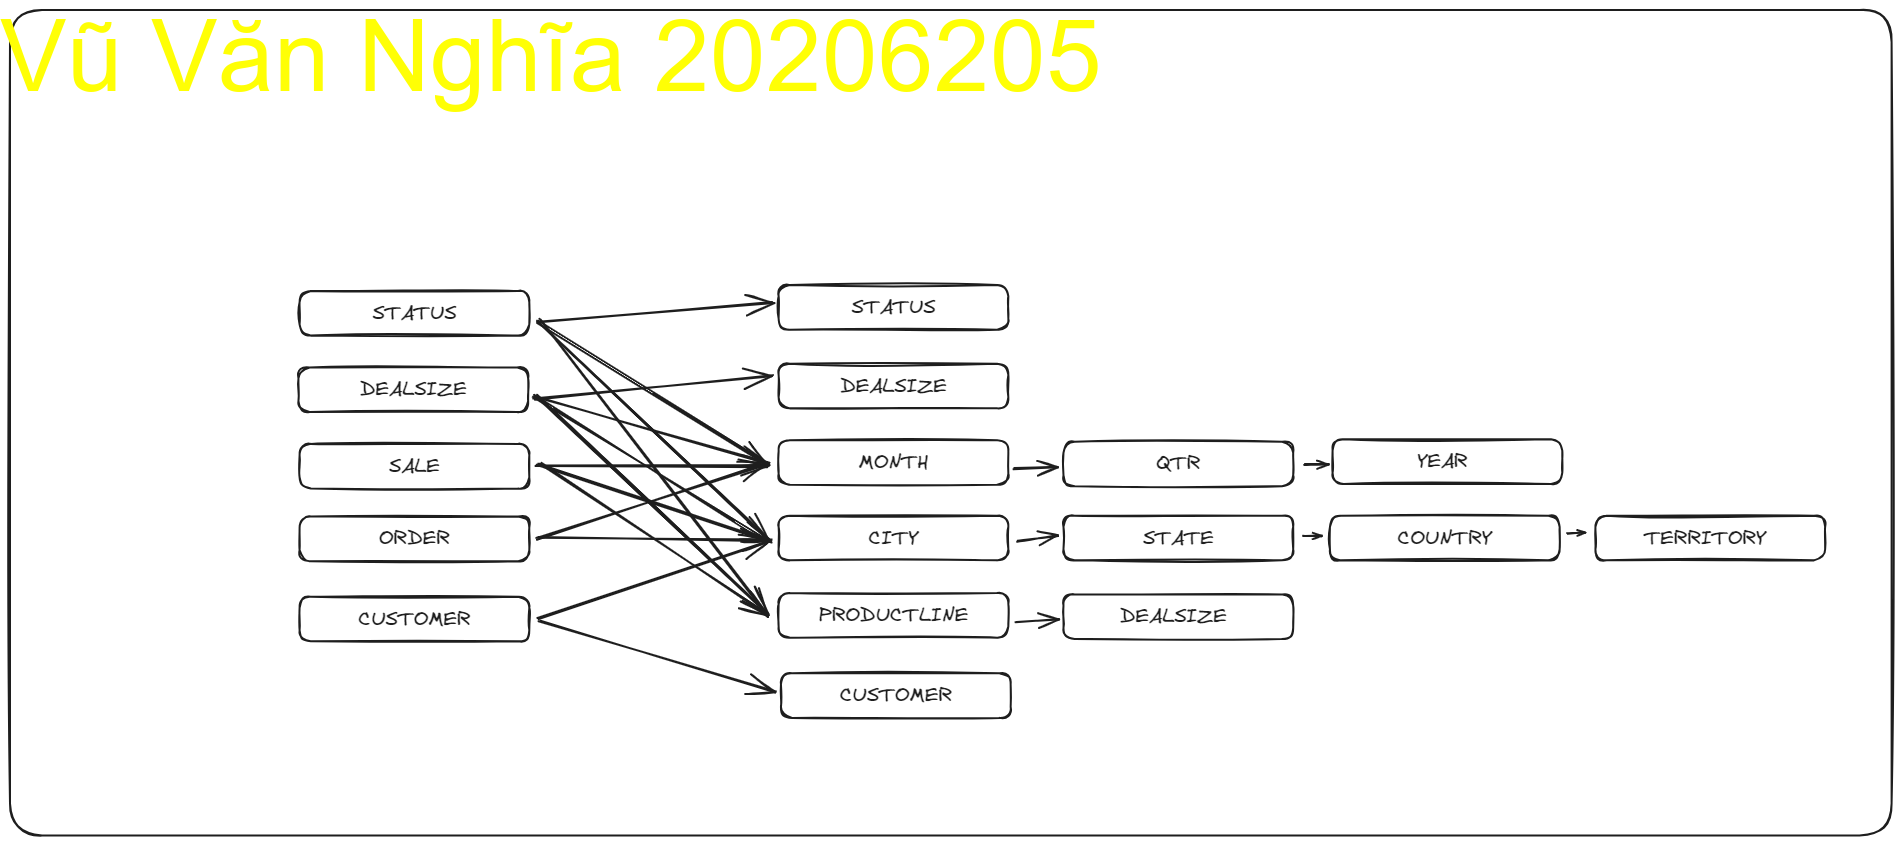
\includegraphics[scale = 0.15]{Bai2/ThucHanh/DIM-FACT.png}
        \caption{Thực hành tạo dashboard}
        \end{figure}
    \subsubsection{ Vẽ voi DIM}
        
       
    \begin{figure}[H]
        \centering
        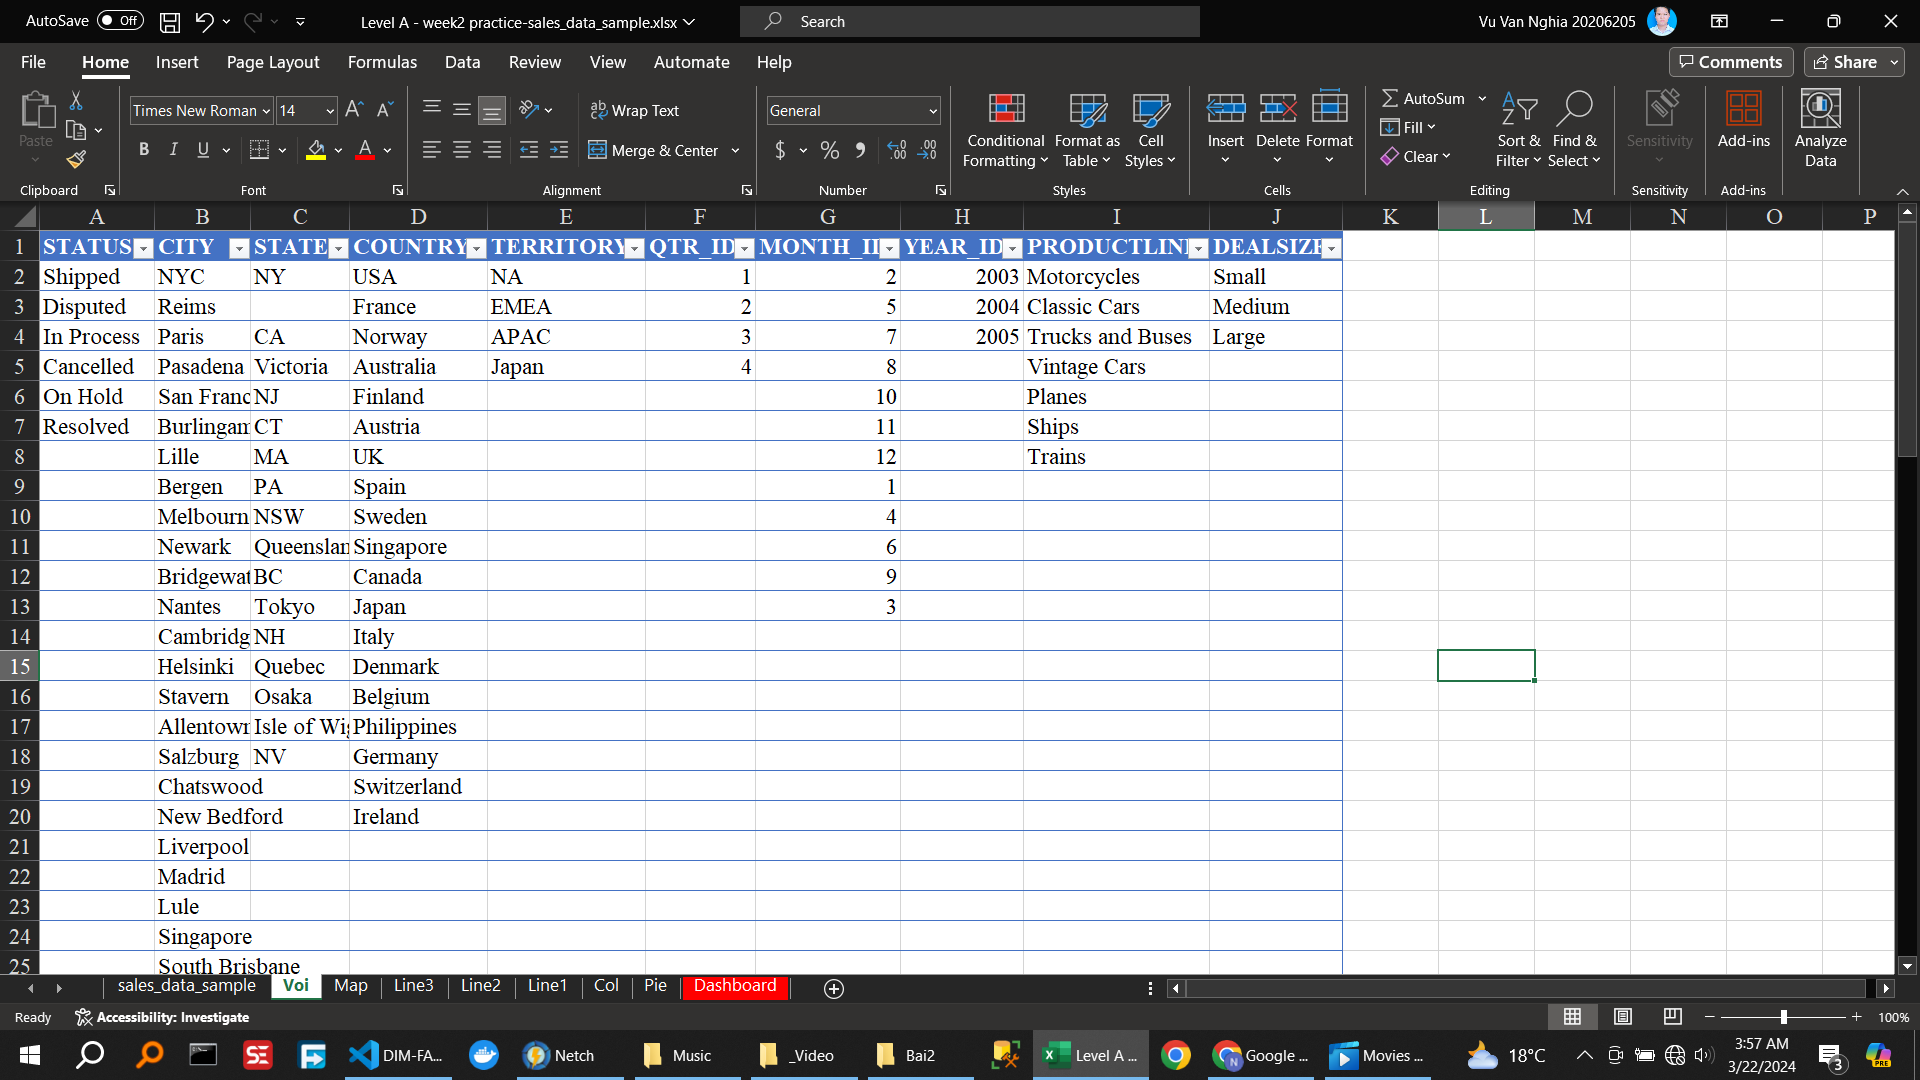
\includegraphics[scale = 0.15]{Bai2/ThucHanh/voi.png}
        \caption{Thực hành tạo dashboard}
        \end{figure}



 \subsubsection{Xây dựng một dashboard trên dữ liệu này theo requirement}

\begin{figure}[H]
\centering
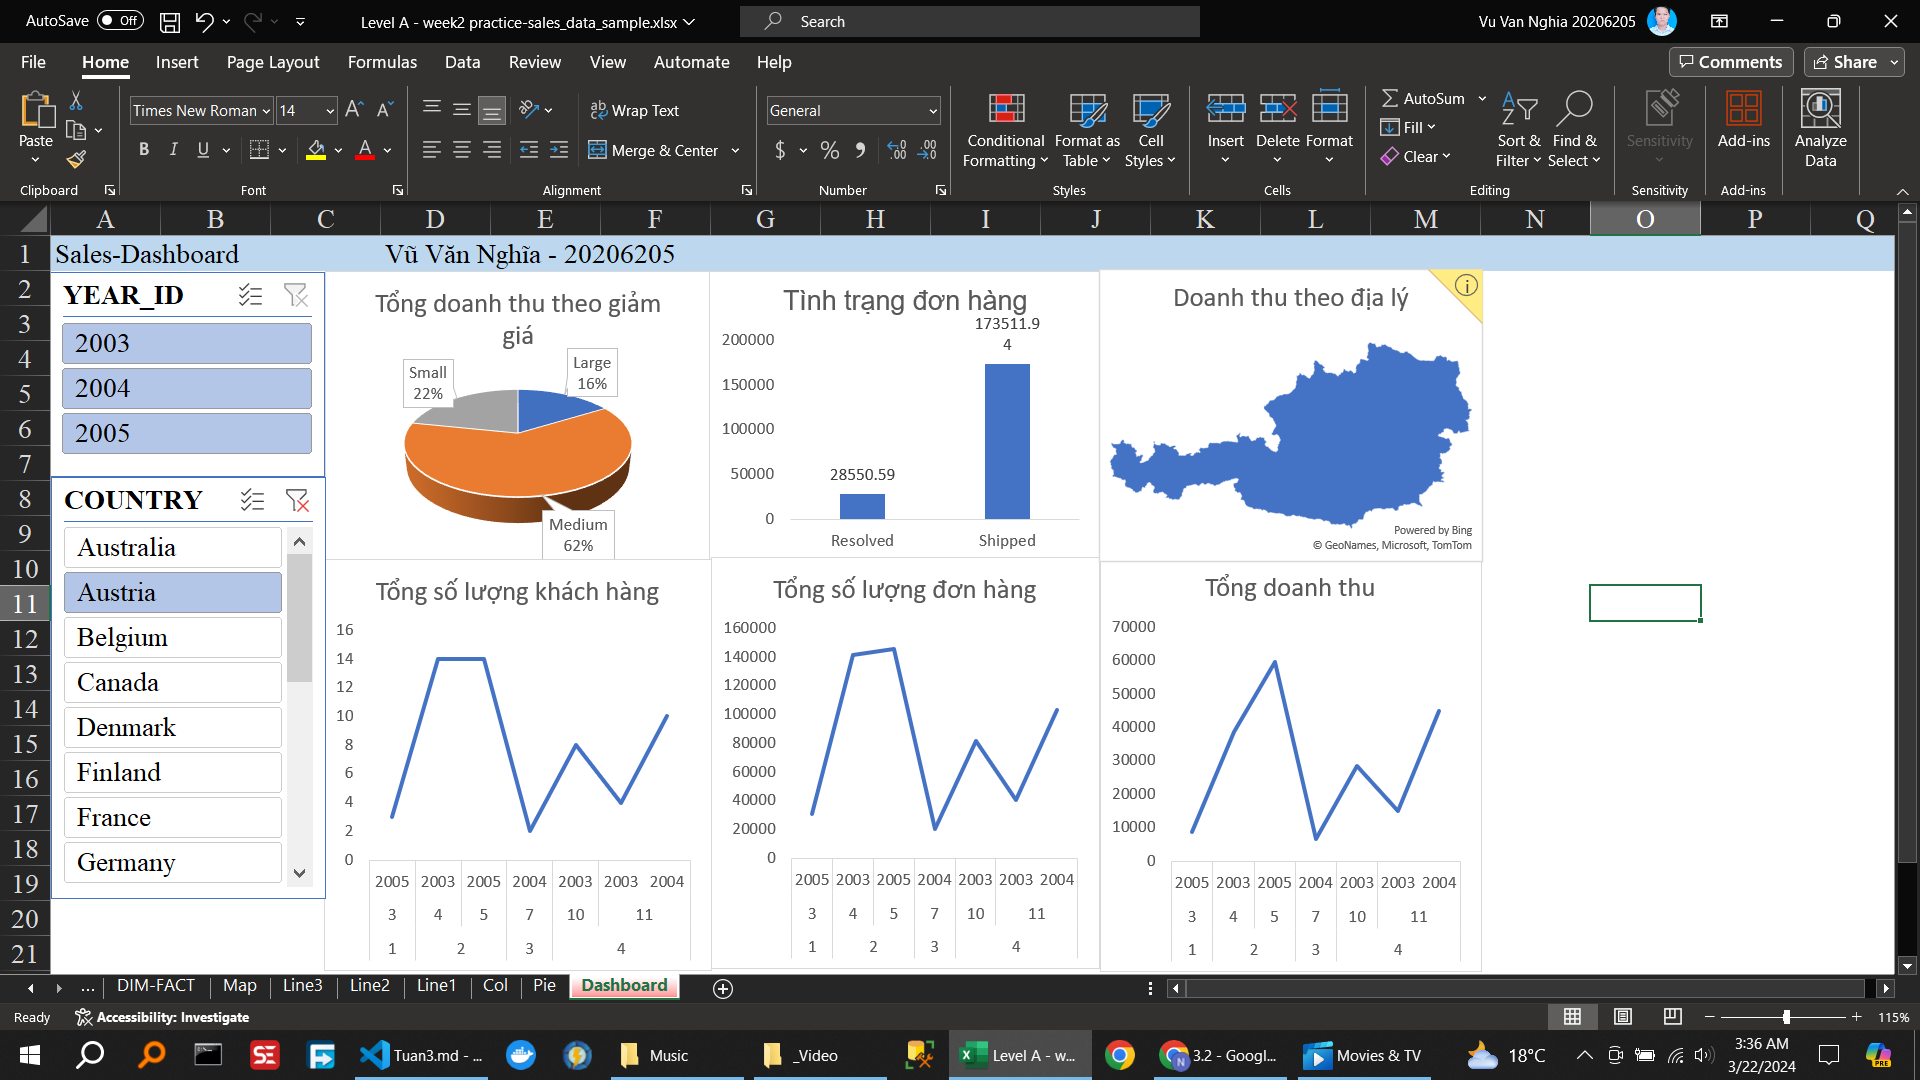
\includegraphics[scale = 0.15]{Bai2/ThucHanh/dashboard.png}
\caption{Thực hành tạo dashboard}
\end{figure}
 




\subsubsection{Phân tích trên dashboard vừa xây dựng}
 
\begin{itemize} 

    \item  Dashboard hiển thị nhiều dữ liệu hữu ích: tổng doanh số bán hàng của công ty mỗi năm từ 2003-2005, có thể lọc theo tháng và quốc gia.
    \item  Doanh số của size trung bình là lớn nhất.
    \item  Ta thấy qua các năm, doanh số tăng nhẹ, điều này là do cuộc sống ngày càng đi lên nên nhu cầu tăng thêm.
  
        \end{itemize} 
%%%%%%%%%%%%%%%%%%%%%%%%%%%%%%%%%%%%%%%%%%%%%%%%%%%%%%%
\end{document}
%%%%%%%%%%%%%%%%%%%%%%%%%%%%%%%%%%%%%%%%%%%%%%%%%%%%%%%